\documentclass[12pt,aspectratio=169]{beamer}
\usepackage{pxfonts}

\usepackage{fancyvrb}
\fvset{%frame=single,
commandchars=\\\{\},
%framesep=1mm,
fontfamily=helvetica,
fontsize=\normalsize
}
%\usepackage[bitstream-charter]{mathdesign}
\usepackage{listings}
\lstset{commentstyle=\color{orange}, keywordstyle=\color{yellow} }

\usepackage{newpxtext}
\usepackage{eulerpx}

\usetheme{Boadilla}
\useoutertheme{split}
\usecolortheme{albatross}


\setbeamertemplate{blocks}[rounded][shadow=false]
\setbeamertemplate{navigation symbols}{}
%\beamerdefaultoverlayspecification{<+->}


\setbeamercolor*{structure}{fg=green!75!black,bg=blue!70!white}
\setbeamercolor*{normal text}{fg=green!65!black,bg=blue!80!black}
\setbeamercolor{palette primary}{use={structure,normal text},fg=green,bg=structure.bg!75!black}
\setbeamercolor{palette secondary}{use={structure,normal text},fg=structure.fg,bg=structure.bg!60!black}
\setbeamercolor{palette tertiary}{use={structure,normal text},fg=structure.fg,bg=structure.bg!45!black}
\setbeamercolor{palette quaternary}{use={structure,normal text},fg=green,bg=structure.bg!75!black}
\setbeamercolor*{example text}{fg=green!65!black}
\setbeamercolor*{block body}{bg=structure.bg!90!black}
\setbeamercolor*{block body alerted}{bg=structure.bg!90!black}
\setbeamercolor*{block body example}{bg=structure.bg!90!black}
\setbeamercolor*{block title}{parent=structure,bg=structure.bg!75!black}
\setbeamercolor*{block title alerted}{use={structure,alerted text},fg=alerted text.fg!75!structure.fg,bg=structure.bg!75!black}
\setbeamertemplate{navigation symbols}{}
\setbeamertemplate{items}[square]
\setbeamercolor{item projected}{fg=white}
\setbeamercolor*{normal text}{fg=white!90!blue,bg=blue!70!black}
\setbeamercolor*{separation line}{}
\setbeamercolor*{fine separation line}{}
\setbeamercolor{alerted text}{fg=green}

\usepackage[italian]{babel}
\usepackage[utf8]{inputenc}
\usepackage{pgf}
\usepackage{verbatim}
\usepackage{inconsolata}
\usepackage{listings}
\lstset{language=C, frame=single,
  basicstyle=\ttfamily,
  numbers=left, numberstyle=\tiny\color{gray},
  numbersep=5pt, fancyvrb=true
}

\usefonttheme{professionalfonts} % using non standard fonts for beamer
\usefonttheme{serif} % default family is serif
% \usepackage{fontspec}
% \setmainfont{Palatino}

\usepackage{pgf}
\usepackage{tikz}
\usepackage{graphicx}
\usetikzlibrary{%
  arrows,
  arrows.meta,
  positioning,
  calc,
  backgrounds,
  chains,
  matrix,
  patterns,
  automata,
  fit,
  graphs,
  decorations,
  decorations.pathmorphing,
  decorations.pathreplacing,
  decorations.markings,
}

\usepgflibrary{shapes,shapes.geometric}


\usepackage{url}
\usepackage{xmpmulti}
% \usepackage{euler}
%\usepackage[T1]{fontenc}
\pdfpagebox5
% \immediate\write18{sh ./vc}
% \input{vc}

\author{Gianluca Della Vedova}
\title{Bioinformatica}
\institute{Univ. Milano--Bicocca\\
  \texttt{https://www.unimib.it/gianluca-della-vedova}}
\date{\today}
%\pgfdeclareimage[height=1cm]{university-logo}{logounimib}
%\logo{\pgfuseimage{university-logo}}


\begin{document}
\begin{frame}
  \titlepage

  \centering
  Alberi evolutivi --- Filogenesi
\end{frame}



\begin{frame}
\frametitle{Alberi evolutivi --- Filogenesi}

\centering
\includegraphics<1>[height=0.55\textheight]{figures/Phylogenetic_tree_legend}

\begin{block}{Alberi etichettati}
etichetta = distanza stimata
\end{block}

\vfill\small
Public domain \url{https://en.wikipedia.org/wiki/File:Phylogenetic_tree.svg}
\end{frame}

\begin{frame}
\frametitle{Distanze}
\centering
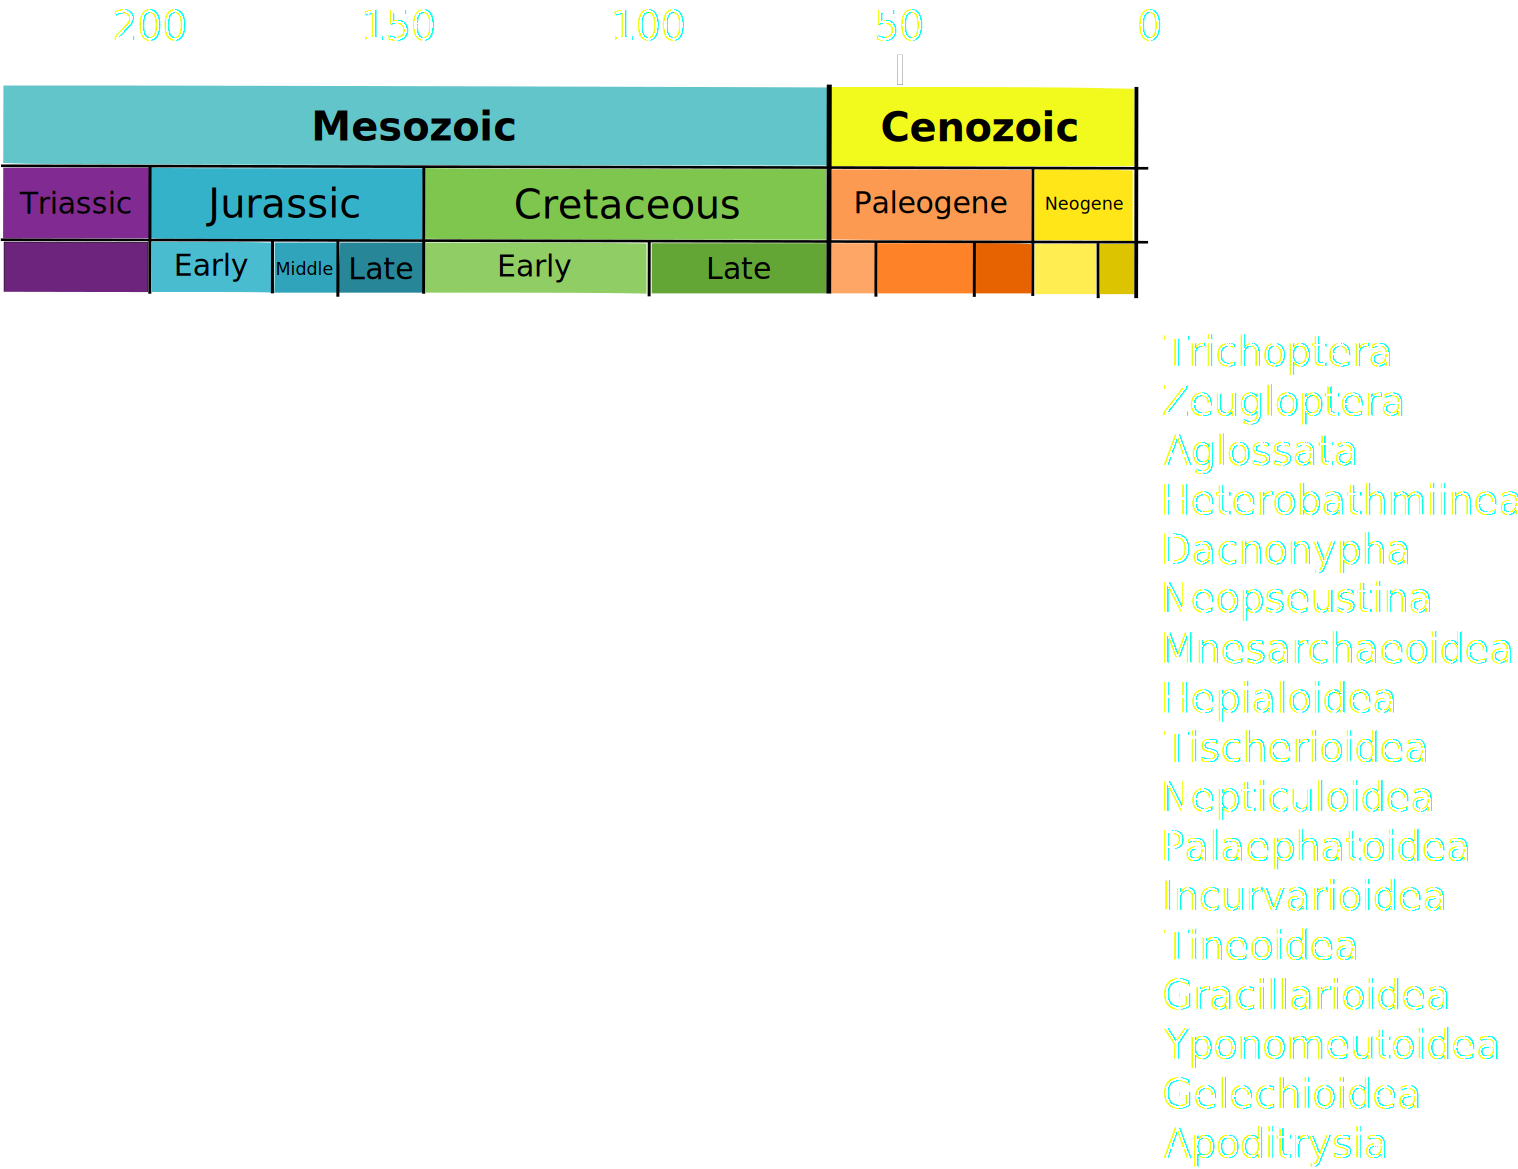
\includegraphics[height=0.95\textheight]{figures/Phylogenetic_chart_of_Lepidoptera_chronogram}
\end{frame}

\begin{frame}
\frametitle{Geni duplicati}
\centering
\includegraphics<1>[width=0.7\textwidth]{figures/Evolution_fate_duplicate_genes}
\end{frame}

\begin{frame}[fragile]
\frametitle{Approcci basati su distanze.}
\begin{block}{Distanza}
$d: S \times S \mapsto \mathbb{R}^{+}$ tale che:
\begin{enumerate}
\item
$d(a,b) = 0 \Leftrightarrow a=b$, $\forall a,b\in S$
\item
$d(a,b) = d(b,a)$, $\forall a,b\in S$ (simmetria)
\item
$d(a,b) \le d(a,c) + d(c,b)$, $\forall a,b,c\in S$ (disuguaglianza triangolare)
\end{enumerate}
\end{block}
\end{frame}



\begin{frame}
\frametitle{Approcci basati su distanze.}
\begin{columns}
  \begin{column}{0.48\textwidth}
{    \scriptsize
 \begin{tabular}{l|cccccc}
        & Sc & A & To & Sa & Ta & L\\ \hline
        Scorpione& - & & & & &\\
        Anguilla& 3 & - & & & &\\
        Tonno& 2 & 1 & - &  & &\\
        Salamandra& 1 & 2 & 1 & - & &\\
        Tartaruga& 3 & 1 & 4 & 1 & -&\\
        Leopardo& 1 & 1 & 1 & 1 & 1 & -
 \end{tabular}
}
\end{column}
  \begin{column}{0.48\textwidth}
\begin{block}{Problema}
  \begin{itemize}
    \item
  Input: matrice $M$ di distanze stimate
    \item
      Output: un albero con le stesse distanze di $M$, se esiste
\end{itemize}
\end{block}
\end{column}
\end{columns}
\end{frame}

\begin{frame}[fragile]
  \frametitle{UPGMA}
\begin{itemize}
\item
  Unweighted Pair Group with Arithmetic Mean
\item
  $D(C_{1}, C_{2}) \gets \frac{1}{|C_{1}||C_{2}|}\sum_{i\in C_{1}}\sum_{j\in C_{2}} D(i,j)$
\item
  All'inizio $h=0$ per ogni cluster/specie
\item
Fondi i due cluster $C_{1}$, $C_{2}$ con minimo $D(\cdot, \cdot)$, ottenendo $C$
\item
  Per ogni cluster $C^{*}\neq C$, $D(C, C^{*}) = \frac{1}{|C||C^{*}|}\sum_{i\in C}\sum_{j\in C^{*}} D(i,j)$
\item
  $h(C)\gets \frac{1}{2}D(C_{1}, C_{2})$
\item
  $h(C) - h(C_{1})$ etichetta $(C, C_{1})$; $h(C) - h(C_{2})$ etichetta $(C, C_{2})$
\item
  UPGMA produce ultrametrica
\end{itemize}
\end{frame}

\begin{frame}[fragile]
\frametitle{Neighbor Joining.}
\begin{itemize}
\item
  $D(C_{1}, C_{2}) \gets \frac{1}{|C_{1}||C_{2}|}\sum_{i\in C_{1}}\sum_{j\in C_{2}} D(i,j)$
\item
  $u(C) \gets \frac{1}{\text{num. cluster} - 2} \sum_{C_{3}} D(C,C_{3})$
\item
  Fondi i due cluster $C_{1}$, $C_{2}$ con minimo $D(C_{1}, C_{2}) - u(C_{1}) -u(C_{2})$, ottenendo $C$
\item
  Per ogni cluster $C^{*}\neq C$, $D(C, C^{*}) = \frac{1}{|C||C^{*}|}\sum_{i\in C}\sum_{j\in C^{*}} D(i,j)$
\item
  $\frac{1}{2}\left(D(C_{1}, C_{2}) + u(C_{1}) - u(C_{2})\right)$ etichetta $(C, C_{1})$
\item
  $\frac{1}{2}\left(D(C_{1}, C_{2}) + u(C_{2}) - u(C_{1})\right)$ etichetta $(C, C_{2})$
\end{itemize}
\end{frame}


\begin{frame}
\frametitle{Evoluzione in un individuo}

\centering
  \includegraphics[width=\linewidth]{figures/progression}
  \begin{itemize}
    \item
      Cellule \alert{accumulano} mutazioni durante la vita
  % \item
  %   Accumulate mutation $\Rightarrow$ perfect phylogeny
  \end{itemize}
\end{frame}




\begin{frame}
\frametitle{Evoluzione basata su caratteri}

\centering
\includegraphics<1>[height=0.55\textheight]{figures/perfect-phylogeny}

\begin{block}{Regola 1 (semplice)}
Ogni carattere è acquisito \alert{esattamente una volta} nell'albero.
\end{block}
\end{frame}


\begin{frame}
  \frametitle{Filogenesi perfetta}
\begin{columns}
  \begin{column}{0.48\textwidth}
{    \scriptsize
 \begin{tabular}{l|ccccc}
        & A & J & H & L & V\\ \hline
        Scorpione& 0 & 0 & 0 & 0 & 0\\
        Anguilla& 0 & 0 & 0 & 0 & 1\\
        Tonno& 0 & 1 & 0 & 0 & 1\\
        Salamandra& 0 & 1 & 0 & 1 & 1\\
        Tartaruga& 1 & 1 & 0 & 1 & 1\\
        Leopardo& 1 & 1 & 1 & 1 & 1
 \end{tabular}
}\begin{block}{Problema}
  \begin{itemize}
    \item
  Input: matrice binaria $M$
    \item
      Output: un albero che \alert{spiega} $M$, se esiste
\end{itemize}
\end{block}

\end{column}

    \begin{column}{0.48\textwidth}
      \centering
\includegraphics<1>[height=0.52\textheight]{figures/perfect-phylogeny}
\end{column}
\end{columns}
\begin{block}{Algorithm di Gusfield --- lineare}
  \begin{enumerate}
    \item
      Radix Sort delle colonne, in ordine decrescente (anche del numero di 1)
    \item
      Costruire l'albero, una specie alla volta
    \end{enumerate}
  \end{block}
\end{frame}




% \begin{frame}
% \frametitle{Losing characters}

% \centering
% \includegraphics<1>[height=0.65\textheight]{figures/classification-of-life-taxonomy}

% \begin{block}{A possible rule}
% Each character can be lost (once).
% \end{block}

% \end{frame}




\begin{frame}
\frametitle{Caratteri e stati}

\begin{block}{Cambio di stato}
  \begin{itemize}
\item  Un carattere $c$ è  \alert{acquisito} $\Rightarrow$ lo stato di  $c$ passa da  $0$ a $1$
  in un arco
  \item  Un carattere $c$ è \alert{perso} $\Rightarrow$   lo stato di  $c$ passa da  $1$ a $0$
  in un arco (\alert{mutazione ricorrente})
\end{itemize}
\end{block}

\begin{block}{Modelli di evoluzione}
Ogni carattere $c$ è  acquisito \alert{esattamente una volta} nell'albero.
\begin{enumerate}
\item
  Filogenesi perfetta: nessuna mutazione ricorrente, nessuna perdita
% \item
%   Filogenesi persistente: ogni carattere può essere perso al massimo una volta nell'albero.
% \alert{modello $012$}
\item
  \alert{Dollo}:
  mutazioni ricorrenti senza limiti, ma senza perdite
\item
  \alert{Camin-Sokal}:
  Perdite senza limiti, ma senza mutazioni ricorrenti
\end{enumerate}
\end{block}
\end{frame}


\begin{frame}
\frametitle{Tumori}
\begin{columns}
\begin{column}{0.75\textwidth}
\centering
\includegraphics[width=0.9\linewidth]{figures/tumor-heterogeneous}
\end{column}
\begin{column}{0.25\textwidth}
\begin{itemize}
\item
Un \alert{tumore} contiene sia cellule cancerose che sane
\item
Un \alert{tumore} è un miscuglio di cloni (sottopopolazioni) diverse.
\end{itemize}
\end{column}
\end{columns}
\end{frame}


\begin{frame}
\frametitle{Evoluzione tumorale}
\begin{columns}
\begin{column}{0.75\textwidth}
\centering
  \includegraphics[width=0.99\linewidth]{figures/clonal}
\end{column}
\begin{column}{0.25\textwidth}
\begin{itemize}
\item I cloni compaiono con numerosità differente nel tumore
\end{itemize}
\end{column}
\end{columns}
\end{frame}


\def\mut#1#2{%
\begin{scope}[shift={#1}]
\node[thick,draw,fill=blue!70,circle, scale=3.5] (#2) {};
\end{scope}
}

\def\muta#1#2{%
\begin{scope}[shift={#1}]
\mut{(0,0)}{#2};
\draw[fill=white] (0,0) circle (.1);
\end{scope}
}

\def\mutb#1#2{%
\begin{scope}[shift={#1}]
\muta{(0,0)}{#2};
\node[fill,color=brown,star, star points=6,scale=0.75] at (45:0.3) {};
\end{scope}
}

\def\mutc#1#2{%
\begin{scope}[shift={#1}]
\muta{(0,0)}{#2};
\node[fill,color=green,regular polygon, regular polygon sides=3,scale=0.65] at (90:0.3) {};
\end{scope}
}

\def\mutd#1#2{%
\begin{scope}[shift={#1}]
\mutc{(0,0)}{#2};
\node[fill,color=red,regular polygon, regular polygon sides=4,scale=0.75] at (0:0.3) {};
\end{scope}
}

\def\mute#1#2{%
\begin{scope}[shift={#1}]
\mutd{(0,0)}{#2};
\node[draw,cross out, draw=pink, very thick,scale=.8] at (180:.3) {};
\end{scope}
}

\def\mutf#1#2{%
\begin{scope}[shift={#1}]
\mutd{(0,0)}{#2};
\node[draw,diamond,scale=0.6, fill,color=blue]  at (270:0.3) {};
\end{scope}
}

\begin{frame}
\frametitle{Evoluzione tumorale}

\begin{columns}
  \begin{column}{0.38\textwidth}
\centering
\resizebox{0.95\textwidth}{!}{\begin{tikzpicture}[,>=triangle 60]
\mutf{(-5,5)}{s5};
\muta{(-5.5,7)}{s4};
\muta{(-4,9)}{s4};

\muta{(-2.4,5.8)}{s4};
\mutb{(-1.2,6.7)}{s1};
\mutb{(-3.5,7)}{s1};
\mutc{(-2,8.2)}{s3};
\mutc{(-0.2,8)}{s3};

\mutc{(-4,2)}{s1};
\mut{(-2.5,2)}{};
\mut{(0.5,3.5)}{};
\mut{(-4.5,3.5)}{};
\mutd{(0.5,1.8)}{s6};
\mute{(-3,3.5)}{s2};
\mutf{(-1.2,3)}{s5};
\mutc{(0.5,5)}{s32};

\draw[rotate=30,thick] (2,7) ellipse (2.8 and 2.1);
\node at (-4,0.5) {Sample 1};
\draw[rotate=0,thick] (-3,2.8) ellipse (2.8 and 1.8);
\node at (-2,10) {Sample 2};
\end{tikzpicture}}
\end{column}
  \begin{column}{0.58\textwidth}

\begin{itemize}
\item Un \alert{campione} contiene diversi cloni
\item Per ogni campione, abbiamo la \alert{frequenza} con cui ogni mutazione appare
\item
  matrice di frequenze $F$
%\item inference of tumoral phylogeny
\end{itemize}

\centering
\resizebox{0.95\textwidth}{!}{\begin{tikzpicture}[scale=0.8]
\draw[fill=white] (3,2) circle (.1);
\node[fill,color=brown,star, star points=6,scale=0.75] at (6,2) {};
\node[fill,color=green,regular polygon, regular polygon sides=3,scale=0.65] at (2,2) {};
\node[draw,cross out, draw=pink, very thick,scale=.8] at (5,2) {};
\node[draw,diamond,scale=0.6, fill,color=blue]  at (1,2) {};
\node[fill,color=red,regular polygon, regular polygon sides=4,scale=0.75] at (4,2) {};

\node at (1,1) {0.2}; \node at (2,1) {0.6}; \node at (3,1) {0.6};
\node at (4,1) {0.4}; \node at (5,1) {0.2}; \node at (6,1) {0.0};
\node at (1,0) {0.0}; \node at (2,0) {0.4}; \node at (3,0) {1.0};
\node at (4,0) {0.0}; \node at (5,0) {0.0}; \node at (6,0) {0.4};

\node at (0,1) {$S_{1}$}; \node at (0,0) {$S_{2}$};
\end{tikzpicture}}

\end{column}
\end{columns}
\end{frame}


\begin{frame}
\frametitle{Calcolare l'evoluzione tumorale}

\begin{columns}
  \begin{column}{0.40\textwidth}
    \begin{block}{Matrice $B$ spiegata da $T$}
    \end{block}
\centering
\resizebox{0.61\textwidth}{!}{\begin{tikzpicture}[scale=0.44]
\draw[fill=white] (3,2) circle (.1);
\node[fill,color=brown,star, star points=6,scale=0.5] at (6,2) {};
\node[fill,color=green,regular polygon, regular polygon sides=3,scale=0.5] at (2,2) {};
\node[draw,cross out, draw=pink, very thick,scale=.6] at (5,2) {};
\node[draw,diamond,scale=0.46, fill,color=blue]  at (1,2) {};
\node[fill,color=red,regular polygon, regular polygon sides=4,scale=0.5] at (4,2) {};
\end{tikzpicture}}
\begin{tabular}{rrrrrr}
    0 & 0 & 1 & 0 & 0 &1  \\
  0 & 1 & 1 & 1 & 1 &0  \\
  0 & 1 & 1 & 0 & 0 &0  \\
  0 & 0 & 1 & 0 & 0 &0  \\
  1 & 1 & 1 & 1 & 0 &0  \\
\end{tabular}
%     \begin{block}{Matrice uso $U$}
%     \end{block}
% \resizebox{0.79\textwidth}{!}{\begin{tabular}{rrrrr}
%      \multicolumn{5}{c}{Specie}\\
%   0 & 0.2 & 0.2 & 0 & 0.2  \\
%   0.4 & 0 & 0.4 & 0.2 & 0   \\
% \end{tabular}}
\end{column}


  \begin{column}{0.42\textwidth}
  \resizebox{\textwidth}{!}{
  \begin{tikzpicture}[>=triangle 60]
    \mut{(3,9.5)}{N};
    \muta{(3,7)}{s4};
    \mutb{(5,0.5)}{s1};
    \mutc{(0,5)}{s3};
\mutd{(-2,2.8)}{s6};
\mute{(-3,0.5)}{s2};
\mutf{(-1,0.5)}{s5};
\mutc{(1,0.5)}{s32};
\muta{(3,0.5)}{s42};
\draw[thick,->,>=stealth] (N) to node[midway, right=5pt,circle, fill, scale=.6] (e1){} node[right=10pt]{}(s4) ;
\draw[thick,->,>=stealth] (s4) to node[near start,right=5pt,fill,color=brown,star, star points=7,scale=0.6]  {}node[right=10pt,near start]{} (s1) ;
\draw[thick,->,>=stealth] (s4) to node[near start,left=5pt,fill,color=green,regular polygon, regular polygon sides=3,scale=0.45]  {} node[left=10pt,near start]{} (s3) ;
\draw[thick,->,>=stealth] (s3) to node[near start,left=5pt,fill,color=red,regular polygon, regular polygon sides=4,scale=0.7]  {} node[left=10pt,near start]{} (s6) ;
\draw[thick,->,>=stealth] (s6) to node[near start,left=5pt,draw,cross out, pink, very thick,scale=.7]  {} node[left=10pt,near start]{} (s2) ;
\draw[thick,->,>=stealth] (s6) to node[near start,right=5pt,fill,diamond,scale=0.5, fill,color=blue]  {} node[right=10pt,near start]{} (s5) ;
\draw[thick,->,>=stealth] (s3) -- (s32) ;
\draw[thick,->,>=stealth] (s4) to   (s42) ;

\draw (-4,-1) rectangle node[pos=.18] {Sample 1}(1.9,1.5);
\draw[dashed] (6,-1.5) rectangle node[yellow, pos=.2] {Sample 2}(0.0,2);
  \end{tikzpicture}
}
\end{column}
\end{columns}
\end{frame}


\begin{frame}[fragile]
  \frametitle{Modelli di evoluzione.}
\begin{itemize}
\item
  Probabilità di transizione fra stati (A, C, G, T).
  %
\item
  dipende dal tempo trascorso fra i due eventi
\item
  tasso istantaneo di mutazione
\item
  probabilità di mutazione \emph{in una generazione}: somma su ogni riga = $1$
\end{itemize}

J.~Felsenstein.
%
 Theoretical Evolutionary Genetics
\end{frame}

\begin{frame}[fragile]
  \frametitle{Modelli di evoluzione: Jukes-Cantor.}
\begin{itemize}
\item
  ogni mutazione è equiprobabile
\item
  $1-\mu$: nessuna mutazione
\item
  $\mu/3$: mutazione
\end{itemize}
\end{frame}

\begin{frame}[fragile]
  \frametitle{Modelli di evoluzione: Kimura 2 parametri}
\begin{itemize}
\item
  Distinzione transizioni ($A\leftrightarrow G$, $C\leftrightarrow T$), transversioni
\item
  $1-\mu$: nessuna mutazione
\item
  $\frac{R}{R+1}\mu$: probabilità transizione
\item
  $\frac{1}{2(R+1)}\mu$: probabilità di trasversione $A\leftrightarrow C$ o $G\leftrightarrow T$
\item
  $\frac{1}{2(R+1)}\mu$: probabilità di trasversione $A\leftrightarrow T$ o $C\leftrightarrow G$
\item
  $R = \frac{R}{R+1}\mu / \left(2 \frac{1}{2(R+1)}\mu \right)$: rapporto probabilità di transizioni / probabilità trasversioni
\end{itemize}
\end{frame}

\begin{frame}[fragile]
  \frametitle{Modelli di evoluzione: General time-reversible}
\begin{itemize}
\item
  matrice simmetrica
\item
  consequenza: alberi senza radice
\end{itemize}
\end{frame}


\begin{frame}[fragile]
\frametitle{Massima verosimiglianza.}
\end{frame}



\begin{frame}[containsverbatim]\frametitle{Licenza d'uso}
  \small

  Quest'opera {\`e} soggetta alla licenza Creative Commons:
Attribuzione-Condividi allo stesso modo 4.0.
  (\verb+https://creativecommons.org/licenses/by-sa/4.0/+).

Sei libero di riprodurre, distribuire, comunicare al pubblico, esporre
in pubblico, rappresentare, eseguire, recitare e modificare quest'opera
alle seguenti condizioni:
\begin{itemize}
\item
Attribuzione — Devi attribuire la paternit{\`a} dell'opera nei modi
indicati dall'autore o da chi ti ha dato l'opera in licenza e in modo tale da
non suggerire che essi avallino te o il modo in cui tu usi l'opera.
\item
Condividi allo stesso modo — Se alteri o trasformi quest'opera, o se
la usi per crearne un'altra, puoi distribuire l'opera risultante solo con
una licenza identica o equivalente a  questa.
\end{itemize}
%  \vspace*{1cm}
\end{frame}

\end{document}
